When having to find the balls, their individual position, number and color it will be easier if the background color (color of the cloth) is removed before doing the other operations. This will be done by finding the dominant color in the image which will be the color of the cloth.


This color will be represented in HSB (Hue Saturation Value) which shoule be more light invariant than using RBG or a similar representation of colors.

The following image will be the test image\ref{fig:poolnofilter}:
\begin{figure}[H]
\begin{center}
\leavevmode
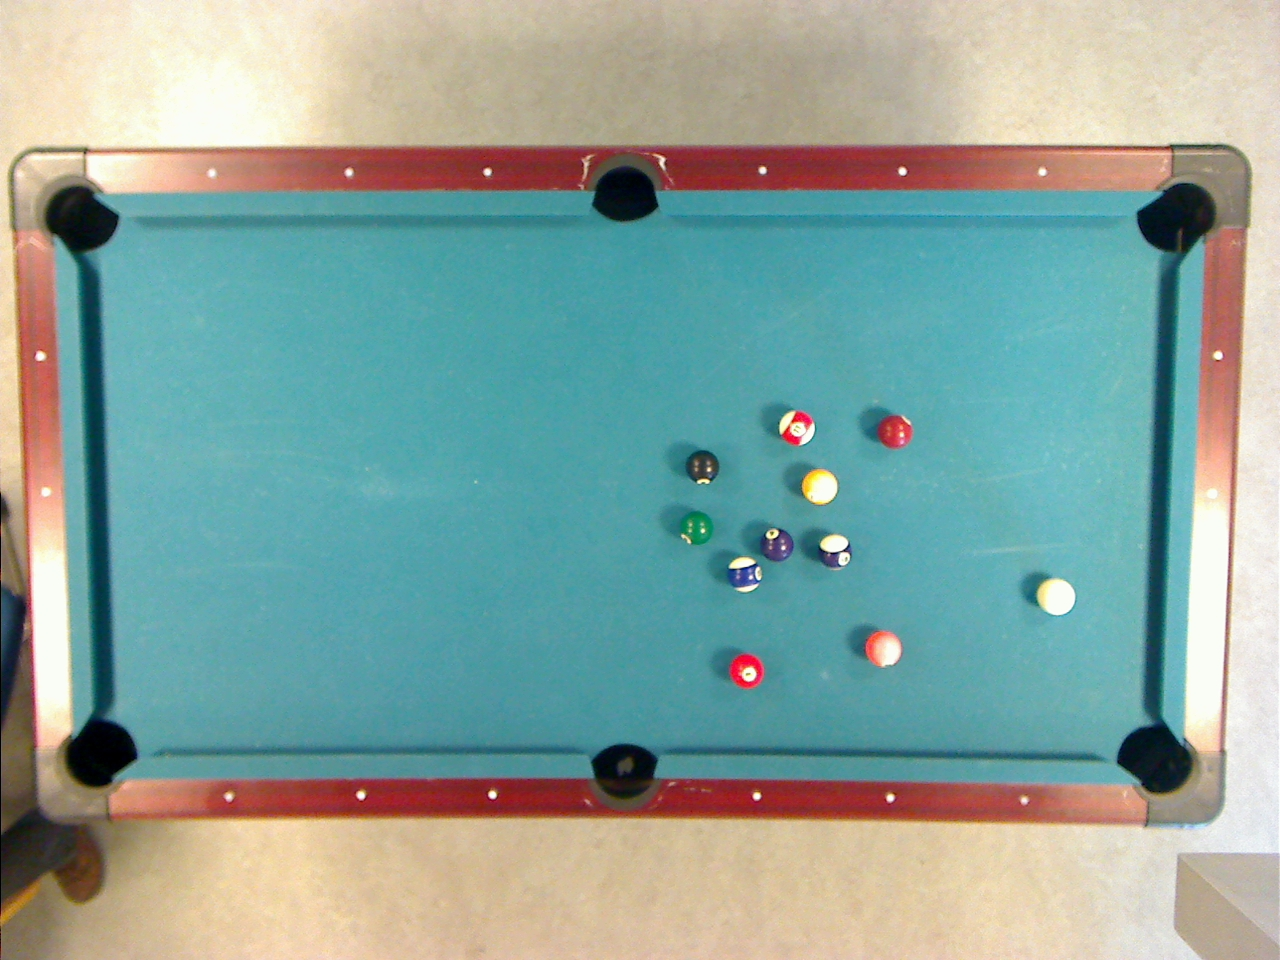
\includegraphics[width=0.8\textwidth]{images/table-no-filters.jpg}
\end{center}
\caption{Pool table with no image processing done.}
\label{fig:poolnofilter}
\end{figure}

A histogram of the image represented pr. pixel in HSB can be seen in \ref{fig:histpoolHSB}. Two histograms were made. One for the full table and sourroundings, and one for only the cloth.
\begin{figure}[H]
\begin{center}
\leavevmode
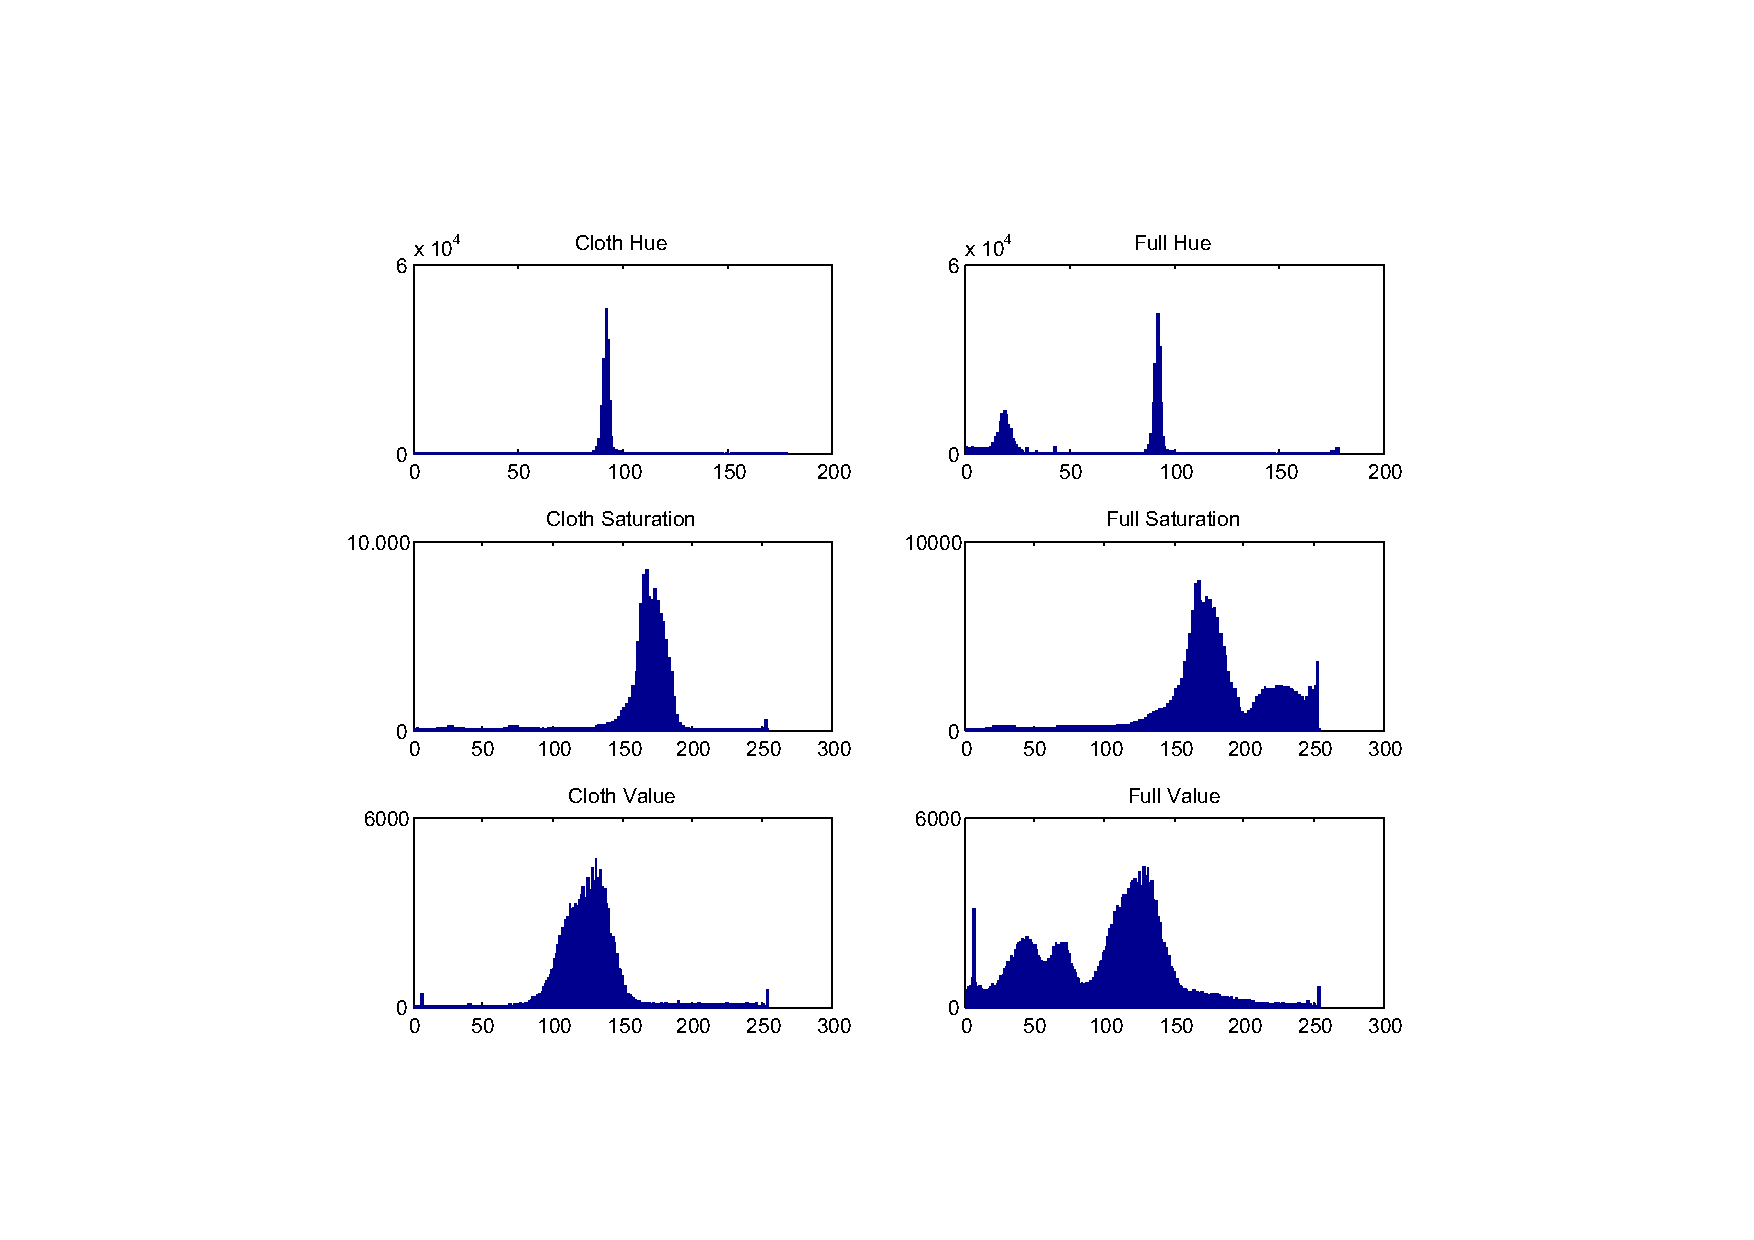
\includegraphics[width=0.8\textwidth]{images/hist2.pdf}
\end{center}
\caption{Histograms of cloth only and full table in HSB.}
\label{fig:histpoolHSB}
\end{figure}

As it can be seen it should be possible to subtract the background without removing too much information about ball location etc. The hue is very easily identified where the saturation and value are broader peaks.
The most common values, calculated in the software, of HSB are (92,129,168) which the histograms also indicate.

By using the following filter we can subtract the pixels in the image that are close to the most common values, more specificly the pixel is identified as being a part of the cloth if following conditions are fulfilled:

Hue is +/- 10 of most common hue-value.\\
Saturation is +/- 50 of most common saturation-value.\\
Value is +/- 50 of most common value-value.\\

The output from this operation can be seen in image\ref{fig:poolclothremoval}.

\begin{figure}[H]
\begin{center}
\leavevmode
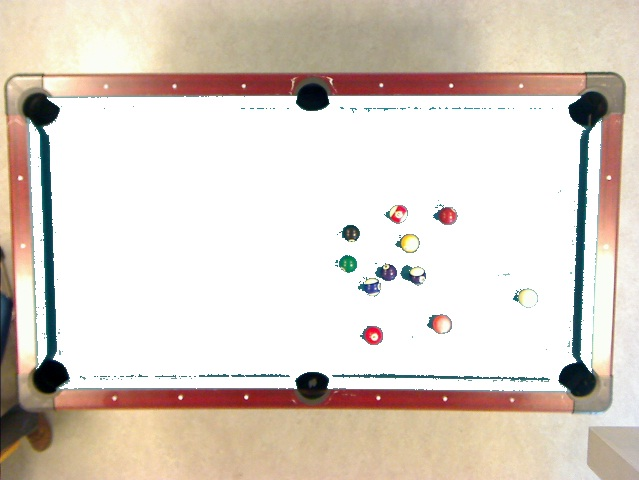
\includegraphics[width=0.8\textwidth]{images/table-remove-cloth.jpg}
\end{center}
\caption{Pool table with cloth removal.}
\label{fig:poolclothremoval}
\end{figure}



